\section{Interoperation Example Between both Approaches}

This section aims to experimentally proof the validity of the alignment presented in the previous section.
To this end, we present two implementations of the same simple scenario.
The goal of the scenario is to remotely change the light of a lamp.

The first implementation uses the proof-based actuation mechanism presented in Section~\ref{}.
The second implementation uses a space-based one.
Then, we mix nodes from the previous implementations and analyse the adjustments required to enable their interoperation.
Sections \ref{sec:actuation_scn1}, \ref{sec:actuation_scn2} and \ref{sec:actuation_scn3} describe these scenarios respectively.
% TODO TODO TODO The implementation is publicly available in URL.



\newcommand{\nodea}{\emph{A} node}
\newcommand{\nodeb}{\emph{B} node}
\newcommand{\nodec}{\emph{C} node}
\newcommand{\noded}{\emph{D} node}


\subsection{Design decisions}

% mejor igual ponerlo después?

% Ontologies used
% explicar por qué hemos modelado así los escenarios?
% por qué con medidas?
% por qué con preferencias?

% TODO explain why like this? why not directly sensors/light?

% por qué no se tienen en cuenta otras características como la localización o lo que sea => por simplificar
%   en el goal se podrían describir


\subsection{Scenario 1}
\label{sec:actuation_scn1}

% poner un diagrama que presente el escenario?
% En ppio no, porque sería muy sencillote, y el flujo del consumidor que es el complejo ya ha sido explicado.

The first scenario presents the following nodes:
\begin{enumerate}[label=\itshape(\alph*\upshape)]
  \item A node which exposes the lamp and its actuators through a \ac{rest} \ac{api}.
	This \ac{api} is described using \restdesc{}. % REST API seguro 100%? por si acaso decir HTTP API?
	To physically change the light value, any client must send an \acs{http} request to the resource which represents the light actuator.
	
  \item A node which directly communicates with the desired provider.
	To discern which provider's resources has to call and how to do it, this implementation reasons to obtain a plan.
	This plan determines how to fulfil the node's initial goal invoking the needed \ac{http} \acsp{api}.
	Figure~\ref{fig:flow_type_c} shows the actions performed by this type of node in detail.
\end{enumerate}



\begin{figure}
        \centering % proporción chachi: 40%, 20% y 20%
	\subfigure[\nodec] {
                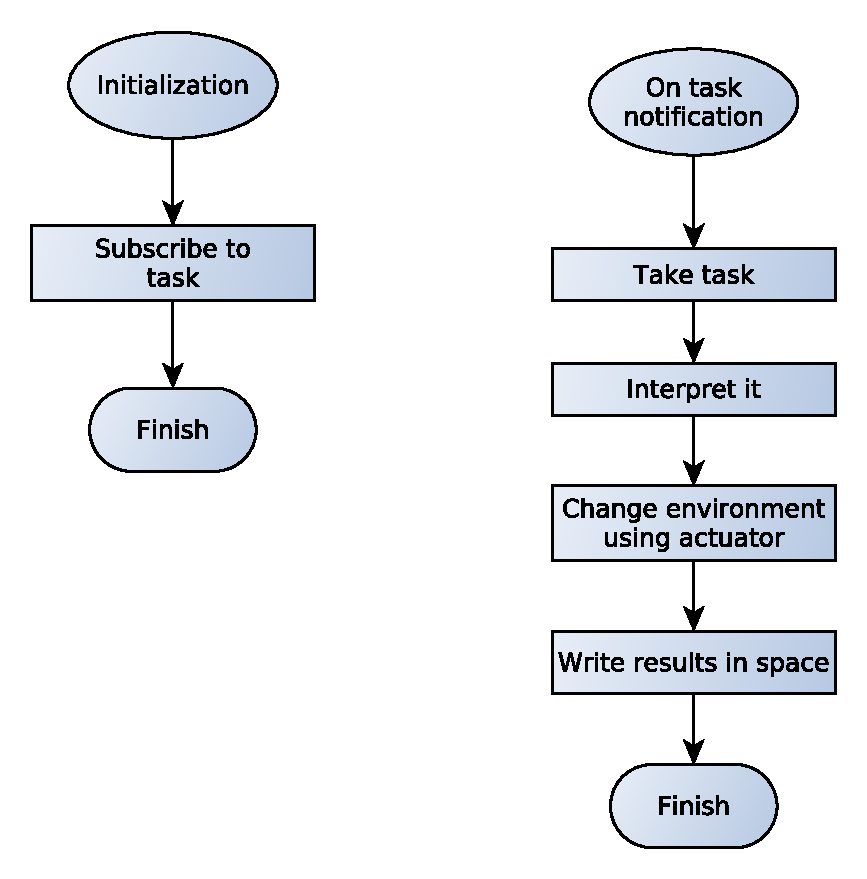
\includegraphics[width=0.22\linewidth]{flowSpaceProvider}
                \label{fig:flow_type_b}
        }
	~ %add desired spacing between images, e. g. ~, \quad, \qquad etc.
          %(or a blank line to force the subfigure onto a new line)
	\subfigure[\noded] {
                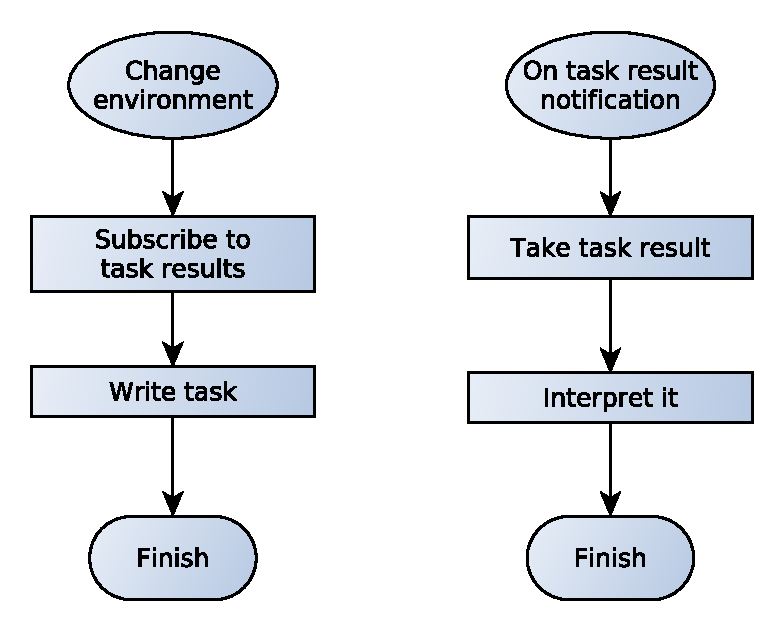
\includegraphics[width=0.22\linewidth]{flowSpaceConsumer}
                \label{fig:flow_type_d}
        }
        ~ %add desired spacing between images, e. g. ~, \quad, \qquad etc.
          %(or a blank line to force the subfigure onto a new line)
        \subfigure[\nodeb] {
                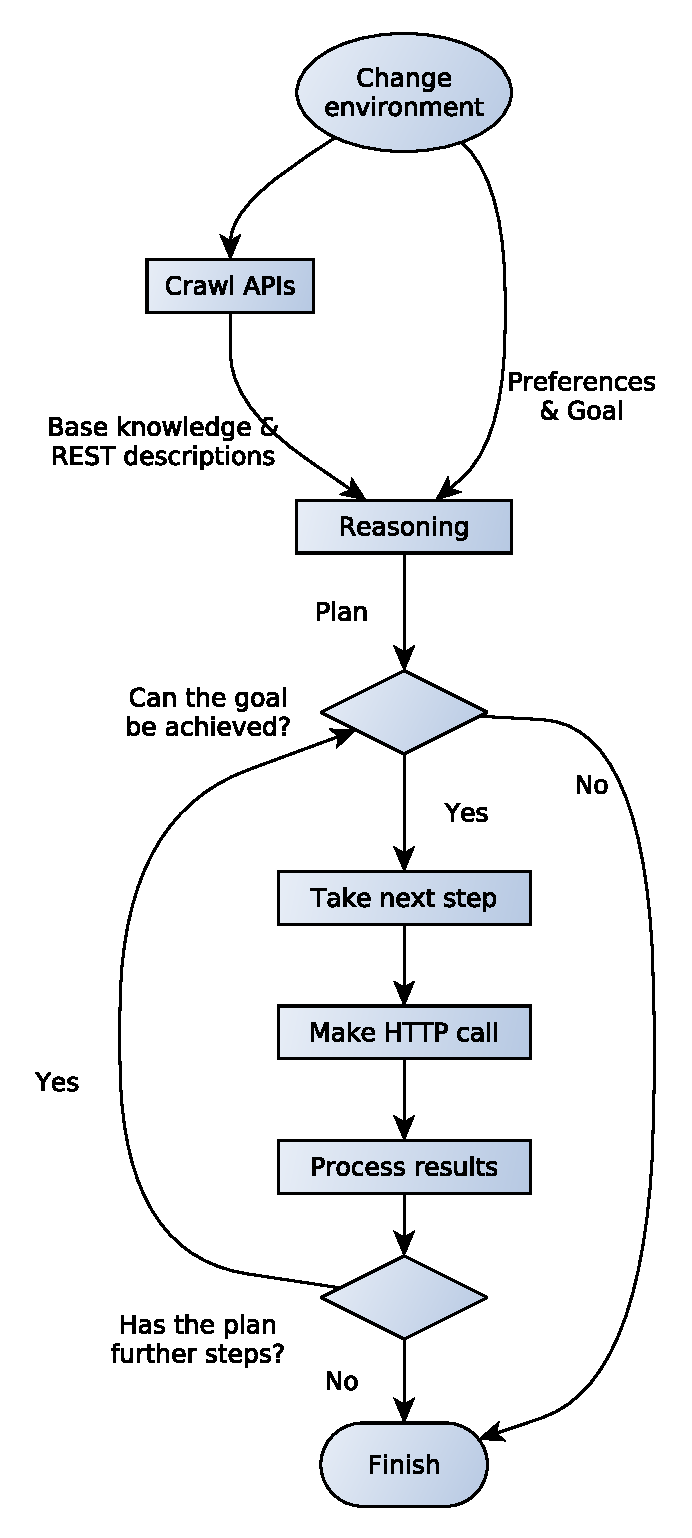
\includegraphics[width=0.44\linewidth]{flowRESTConsumer}
                \label{fig:flow_type_c}
        }%        
        \caption{Flow charts for the different types of nodes.}
        {Please note that \nodea{} is omitted because its operation is the usual for an \acs{http} server.} % actions, behavior, operation???
        \label{fig:flow_nodes}
\end{figure}



The \acs{http} \acs{api} provided by the \nodea{} is modelled using the following resources:
\begin{itemize}
  \item \emph{/lamp}: It provides basic information about the lamp.
  \item \emph{/lamp/actuators}: It enumerates the actuators which compose the \emph{smart lamp}.
  \item \emph{/lamp/actuators/light}: It represents the unique actuator which composes the lamp in our simple example: a light.
  \item \emph{/lamp/actuators/light/01}: It represents a concrete preference to change the light.
\end{itemize}


% Aquí estoy explicando un poco el diagrama de flujo de la figura,
% dando detalles de cómo se ha implementado y a qué me refiero con cada pieza de información
% ¿Añadir descripciones y demás aquí o ponerlas como anexo?

In order to instruct consumers on how to use the services provided, they are annotated using \restdesc{}.
The \acs{http} OPTIONS returns listings~\ref{lst:light_descpost}~and~\ref{lst:measure_descget} for \emph{/lamp/actuators/light}.
Thanks to these descriptions and to the dereferenceable \acsp{uri} \citep{sauermann_cool_2008}, starting from \emph{/lamp} a crawler can autonomously learn how to use the \acs{api}. % TODO citar http://en.wikipedia.org/wiki/Dereferenceable_Uniform_Resource_Identifier
% TODO TODO TODO citar a SIMON!


\begin{listing}
  \expandafter\def\csname PY@tok@err\endcsname{}
{\small
\begin{Verbatim}[commandchars=\\\{\},numbers=left,firstnumber=1,stepnumber=1]
\PY{err}{\PYZob{}}
\PY{n+nc}{  actuators:light }\PY{o}{ssn:madeObservation }\PY{err}{?}\PY{n+na}{l}\PY{n+na}{i}\PY{n+na}{g}\PY{n+na}{h}\PY{n+na}{t}\PY{n+na}{\PYZus{}}\PY{n+na}{o}\PY{n+na}{b}\PY{n+na}{s }.
\PY{err}{\PYZcb{}}\PY{err}{ }\PY{err}{=}\PY{err}{\PYZgt{}}\PY{err}{ }\PY{err}{\PYZob{}}
\PY{n+nc}{  \PYZus{}:request }\PY{o}{http:methodName }\PY{l+s}{\PYZdq{}GET\PYZdq{} };
            \PY{o}{http:requestURI }\PY{err}{?}\PY{n+na}{l}\PY{n+na}{i}\PY{n+na}{g}\PY{n+na}{h}\PY{n+na}{t}\PY{n+na}{\PYZus{}}\PY{n+na}{o}\PY{n+na}{b}\PY{n+na}{s };
            \PY{c}{\PYZsh{}http:body actuators:light ;}
\PY{o}{            http:resp }[\PY{o}{ http:body }\PY{err}{?}\PY{n+na}{l}\PY{n+na}{i}\PY{n+na}{g}\PY{n+na}{h}\PY{n+na}{t}\PY{n+na}{\PYZus{}}\PY{n+na}{o}\PY{n+na}{b}\PY{n+na}{s }].
  
  \PY{err}{?}\PY{n+nc}{light\PYZus{}obs }\PY{o}{a  }\PY{n+na}{s}\PY{n+na}{s}\PY{n+na}{n}\PY{n+na}{:}\PY{n+na}{O}\PY{n+na}{b}\PY{n+na}{s}\PY{n+na}{e}\PY{n+na}{r}\PY{n+na}{v}\PY{n+na}{a}\PY{n+na}{t}\PY{n+na}{i}\PY{n+na}{o}\PY{n+na}{n };
         \PY{o}{ssn:observedProperty  }\PY{n+na}{s}\PY{n+na}{w}\PY{n+na}{e}\PY{n+na}{e}\PY{n+na}{t}\PY{n+na}{:}\PY{n+na}{L}\PY{n+na}{i}\PY{n+na}{g}\PY{n+na}{h}\PY{n+na}{t };
         \PY{o}{ssn:observedBy }\PY{n+na}{a}\PY{n+na}{c}\PY{n+na}{t}\PY{n+na}{u}\PY{n+na}{a}\PY{n+na}{t}\PY{n+na}{o}\PY{n+na}{r}\PY{n+na}{s}\PY{n+na}{:}\PY{n+na}{l}\PY{n+na}{i}\PY{n+na}{g}\PY{n+na}{h}\PY{n+na}{t };
         \PY{o}{ssn:observationResult }\PY{err}{?}\PY{n+na}{s}\PY{n+na}{o }.
     
  \PY{err}{?}\PY{n+nc}{so }\PY{o}{ssn:hasValue }\PY{err}{?}\PY{n+na}{o}\PY{n+na}{v }.

  \PY{err}{?}\PY{n+nc}{ov }\PY{o}{a }\PY{n+na}{s}\PY{n+na}{s}\PY{n+na}{n}\PY{n+na}{:}\PY{n+na}{O}\PY{n+na}{b}\PY{n+na}{s}\PY{n+na}{e}\PY{n+na}{r}\PY{n+na}{v}\PY{n+na}{a}\PY{n+na}{t}\PY{n+na}{i}\PY{n+na}{o}\PY{n+na}{n}\PY{n+na}{V}\PY{n+na}{a}\PY{n+na}{l}\PY{n+na}{u}\PY{n+na}{e };
      \PY{o}{dul:isClassifiedBy  }\PY{n+na}{u}\PY{n+na}{c}\PY{n+na}{u}\PY{n+na}{m}\PY{n+na}{:}\PY{n+na}{l}\PY{n+na}{u}\PY{n+na}{x };
      \PY{o}{dul:hasDataValue }\PY{n+na}{\PYZus{}}\PY{n+na}{:}\PY{n+na}{v}\PY{n+na}{a}\PY{n+na}{l }.
\PY{err}{\PYZcb{}}\PY{err}{.}
\end{Verbatim}
}
  \caption{Rule which expresses that having a light sensor observation, one can obtain details about the observation through an \acs{http} GET.}
  \label{lst:measure_descget}
\end{listing}

\begin{listing}
  \expandafter\def\csname PY@tok@err\endcsname{}
\begin{Verbatim}[commandchars=\\\{\},numbers=left,firstnumber=1,stepnumber=1]
\PY{err}{\PYZob{}}
\PY{c}{  \PYZsh{} it is not \PYZsq{}just a measure\PYZsq{}}
\PY{err}{ }\PY{err}{ }\PY{err}{?}\PY{n+nc}{obsv }\PY{o}{a }\PY{n+na}{s}\PY{n+na}{s}\PY{n+na}{n}\PY{n+na}{:}\PY{n+na}{O}\PY{n+na}{b}\PY{n+na}{s}\PY{n+na}{e}\PY{n+na}{r}\PY{n+na}{v}\PY{n+na}{a}\PY{n+na}{t}\PY{n+na}{i}\PY{n+na}{o}\PY{n+na}{n}\PY{n+na}{V}\PY{n+na}{a}\PY{n+na}{l}\PY{n+na}{u}\PY{n+na}{e };
      \PY{c}{\PYZsh{} it is also a preference}
\PY{o}{      a }\PY{n+na}{f}\PY{n+na}{r}\PY{n+na}{a}\PY{n+na}{p}\PY{n+na}{:}\PY{n+na}{P}\PY{n+na}{r}\PY{n+na}{e}\PY{n+na}{f}\PY{n+na}{e}\PY{n+na}{r}\PY{n+na}{e}\PY{n+na}{n}\PY{n+na}{c}\PY{n+na}{e };
      \PY{o}{dul:isClassifiedBy  }\PY{n+na}{u}\PY{n+na}{c}\PY{n+na}{u}\PY{n+na}{m}\PY{n+na}{:}\PY{n+na}{l}\PY{n+na}{u}\PY{n+na}{x };
      \PY{o}{dul:hasDataValue }\PY{err}{?}\PY{n+na}{d}\PY{n+na}{e}\PY{n+na}{s}\PY{n+na}{i}\PY{n+na}{r}\PY{n+na}{e}\PY{n+na}{d}\PY{n+na}{\PYZus{}}\PY{n+na}{v}\PY{n+na}{a}\PY{n+na}{l}\PY{n+na}{u}\PY{n+na}{e }.
\PY{err}{\PYZcb{}}\PY{err}{ }\PY{err}{=}\PY{err}{\PYZgt{}}\PY{err}{ }\PY{err}{\PYZob{}}
\PY{n+nc}{  \PYZus{}:request }\PY{o}{http:methodName }\PY{l+s}{\PYZdq{}POST\PYZdq{}};
            \PY{o}{http:requestURI }\PY{n+na}{a}\PY{n+na}{c}\PY{n+na}{t}\PY{n+na}{u}\PY{n+na}{a}\PY{n+na}{t}\PY{n+na}{o}\PY{n+na}{r}\PY{n+na}{s}\PY{n+na}{:}\PY{n+na}{l}\PY{n+na}{i}\PY{n+na}{g}\PY{n+na}{h}\PY{n+na}{t };
            \PY{o}{http:body }\PY{err}{?}\PY{n+na}{d}\PY{n+na}{e}\PY{n+na}{s}\PY{n+na}{i}\PY{n+na}{r}\PY{n+na}{e}\PY{n+na}{d}\PY{n+na}{\PYZus{}}\PY{n+na}{v}\PY{n+na}{a}\PY{n+na}{l}\PY{n+na}{u}\PY{n+na}{e };
            \PY{o}{http:resp }[\PY{o}{ http:body }\PY{err}{?}\PY{n+na}{l}\PY{n+na}{i}\PY{n+na}{g}\PY{n+na}{h}\PY{n+na}{t}\PY{n+na}{O}\PY{n+na}{b}\PY{n+na}{s }].
  
  \PY{n+nc}{actuators:light }\PY{o}{ssn:madeObservation }\PY{err}{?}\PY{n+na}{l}\PY{n+na}{i}\PY{n+na}{g}\PY{n+na}{h}\PY{n+na}{t}\PY{n+na}{O}\PY{n+na}{b}\PY{n+na}{s }.
  
  \PY{err}{?}\PY{n+nc}{lightObs }\PY{o}{a }\PY{n+na}{s}\PY{n+na}{s}\PY{n+na}{n}\PY{n+na}{:}\PY{n+na}{O}\PY{n+na}{b}\PY{n+na}{s}\PY{n+na}{e}\PY{n+na}{r}\PY{n+na}{v}\PY{n+na}{a}\PY{n+na}{t}\PY{n+na}{i}\PY{n+na}{o}\PY{n+na}{n };
         \PY{o}{ssn:observedProperty }\PY{n+na}{s}\PY{n+na}{w}\PY{n+na}{e}\PY{n+na}{e}\PY{n+na}{t}\PY{n+na}{:}\PY{n+na}{L}\PY{n+na}{i}\PY{n+na}{g}\PY{n+na}{h}\PY{n+na}{t };
         \PY{o}{ssn:observedBy }\PY{n+na}{a}\PY{n+na}{c}\PY{n+na}{t}\PY{n+na}{u}\PY{n+na}{a}\PY{n+na}{t}\PY{n+na}{o}\PY{n+na}{r}\PY{n+na}{s}\PY{n+na}{:}\PY{n+na}{l}\PY{n+na}{i}\PY{n+na}{g}\PY{n+na}{h}\PY{n+na}{t };
         \PY{o}{ssn:observationResult }\PY{err}{?}\PY{n+na}{s}\PY{n+na}{o }.
     
  \PY{err}{?}\PY{n+nc}{so }\PY{o}{ssn:hasValue }\PY{err}{?}\PY{n+na}{o}\PY{n+na}{v }.

  \PY{err}{?}\PY{n+nc}{ov }\PY{o}{a }\PY{n+na}{s}\PY{n+na}{s}\PY{n+na}{n}\PY{n+na}{:}\PY{n+na}{O}\PY{n+na}{b}\PY{n+na}{s}\PY{n+na}{e}\PY{n+na}{r}\PY{n+na}{v}\PY{n+na}{a}\PY{n+na}{t}\PY{n+na}{i}\PY{n+na}{o}\PY{n+na}{n}\PY{n+na}{V}\PY{n+na}{a}\PY{n+na}{l}\PY{n+na}{u}\PY{n+na}{e };
      \PY{o}{dul:isClassifiedBy }\PY{n+na}{u}\PY{n+na}{c}\PY{n+na}{u}\PY{n+na}{m}\PY{n+na}{:}\PY{n+na}{l}\PY{n+na}{u}\PY{n+na}{x };
      \PY{o}{dul:hasDataValue }\PY{err}{?}\PY{n+na}{d}\PY{n+na}{e}\PY{n+na}{s}\PY{n+na}{i}\PY{n+na}{r}\PY{n+na}{e}\PY{n+na}{d}\PY{n+na}{\PYZus{}}\PY{n+na}{v}\PY{n+na}{a}\PY{n+na}{l}\PY{n+na}{u}\PY{n+na}{e }.
\PY{err}{\PYZcb{}}\PY{err}{.}
\end{Verbatim}

  \caption{Rule which expresses that having a preference which is measured in luxes, one can create a light observation using the \acs{http} POST.}
  \label{lst:light_descpost}
\end{listing}


In addition to the crawled content, the \nodeb{} provides two extra pieces of information to the reasoner: a preference and a goal (see listings~\ref{lst:additional_information} and~\ref{lst:light_goal}).
The preference allows the consumer express the interest on change a service, which may not always be feasible.
The goal drives the reasoning, which tries to extract a plan to achieve it.

\begin{listing}
  \expandafter\def\csname PY@tok@err\endcsname{}
\begin{Verbatim}[commandchars=\\\{\},numbers=left,firstnumber=1,stepnumber=1]
\PY{k}{@prefix }\PY{n+nv}{frap:  }\PY{n+nn}{\PYZlt{}http://purl.org/frap/\PYZgt{} .}
\PY{k}{@prefix }\PY{n+nv}{dul:  }\PY{n+nn}{\PYZlt{}http://www.loa.istc.cnr.it/ontologies/DUL.owl\PYZsh{}\PYZgt{} .}
\PY{k}{@prefix }\PY{n+nv}{ssn:  }\PY{n+nn}{\PYZlt{}http://www.w3.org/2005/Incubator/ssn/ssnx/ssn\PYZsh{}\PYZgt{} .}
\PY{k}{@prefix }\PY{n+nv}{ucum:  }\PY{n+nn}{\PYZlt{}http://purl.oclc.org/NET/muo/ucum/\PYZgt{} .}
\PY{k}{@prefix }\PY{n+nv}{: }\PY{n+nn}{\PYZlt{}http://example.org/lamp/\PYZgt{}.}


\PY{c}{\PYZsh{} Description of the preference}
\PY{n+nc}{:obsv }\PY{o}{a }\PY{n+na}{s}\PY{n+na}{s}\PY{n+na}{n}\PY{n+na}{:}\PY{n+na}{O}\PY{n+na}{b}\PY{n+na}{s}\PY{n+na}{e}\PY{n+na}{r}\PY{n+na}{v}\PY{n+na}{a}\PY{n+na}{t}\PY{n+na}{i}\PY{n+na}{o}\PY{n+na}{n}\PY{n+na}{V}\PY{n+na}{a}\PY{n+na}{l}\PY{n+na}{u}\PY{n+na}{e}\PY{err}{,}\PY{n+na}{ f}\PY{n+na}{r}\PY{n+na}{a}\PY{n+na}{p}\PY{n+na}{:}\PY{n+na}{P}\PY{n+na}{r}\PY{n+na}{e}\PY{n+na}{f}\PY{n+na}{e}\PY{n+na}{r}\PY{n+na}{e}\PY{n+na}{n}\PY{n+na}{c}\PY{n+na}{e };
      \PY{o}{dul:isClassifiedBy  }\PY{n+na}{u}\PY{n+na}{c}\PY{n+na}{u}\PY{n+na}{m}\PY{n+na}{:}\PY{n+na}{l}\PY{n+na}{u}\PY{n+na}{x };
      \PY{o}{dul:hasDataValue }\PY{n+na}{1}\PY{n+na}{9 }. 
\end{Verbatim}

  \caption{A preference which expresses the interest on modifying the sensed value of a light.}
  \label{lst:additional_information}
\end{listing}

\begin{listing}
  \expandafter\def\csname PY@tok@err\endcsname{}
{\small
\begin{Verbatim}[commandchars=\\\{\},numbers=left,firstnumber=1,stepnumber=1]
\PY{p}{\PYZob{}}
  \PY{c}{\PYZsh{} More things could be specified.}
  \PY{c}{\PYZsh{} E.g. location.}
  
  \PY{n+nc}{actuators:light} \PY{n+nf}{ssn:madeObservation} \PY{n+nv}{?light} \PY{p}{.}
  
  \PY{n+nv}{?light} \PY{n+nf}{ssn:observedProperty}  \PY{n+na}{sweet:Light} \PY{p}{;}
         \PY{n+nf}{ssn:observationResult} \PY{n+nv}{?so} \PY{p}{.}
  
  \PY{n+nv}{?so} \PY{n+nf}{ssn:hasValue} \PY{n+nv}{?ov} \PY{p}{.}
  
  \PY{n+nv}{?ov} \PY{o}{a} \PY{n+na}{ssn:ObservationValue} \PY{p}{;}
      \PY{n+nf}{dul:isClassifiedBy}  \PY{n+na}{ucum:lux} \PY{p}{;}
      \PY{n+nf}{dul:hasDataValue} \PY{l+m+mi}{19} \PY{p}{.}
\PY{p}{\PYZcb{}} \PY{o}{=\PYZgt{}} \PY{p}{\PYZob{}}
  \PY{n+nv}{?ov}  \PY{n+nf}{dul:hasDataValue}  \PY{n+nv}{?val} \PY{p}{.}
\PY{p}{\PYZcb{}}\PY{p}{.}
\end{Verbatim}
}
  \caption{A goal which expresses the interest on modifying the value for a light.}
  \label{lst:light_goal}
\end{listing}

With that plan, the consumer just needs to complete it calling to different \acs{http} resources.
If more than a resource needs to be called, the plan may also indicate how to use the information obtained from one to use it in the next call.


\subsection{Scenario 2}
\label{sec:actuation_scn2}

% poner un diagrama que presente el escenario

The second scenario presents the following nodes:
\begin{enumerate}[resume,label=\itshape(\alph*\upshape)]
  \item A node which reacts to the tasks written into a shared semantic space.
	The node running this implementation is aware of the tasks written into the space and changes the light's value accordingly. % esto es, se suscribe a ellas
	Figure~\ref{fig:flow_type_b} shows the initialization of this type node and the process performed when a graph is detected.
	
  \item A node which writes tasks into a shared semantic space describing its desire to change the light's value.
	Figure~\ref{fig:flow_type_d} shows the actions taken by this type of node.
	As it can be seen, the process is divided in two temporarily independent processes.
	The first writes the task and the second processes the result whenever it is written in the space.
\end{enumerate}


\nodec{} first subscribes to changes in the space (see Listing~\ref{lst:task_subscription}).
Then, \noded{} writes a task to be performed (see Listing~\ref{lst:task}) and subscribes to its result.
As a consequence of the writing, \nodec{} reacts by taking the task, interpreting it, changing the environment through its actuator and writing the result.
Finally, \noded{} gets a notification of the written result, takes it and processes it.


\begin{listing}
  \expandafter\def\csname PY@tok@err\endcsname{}
{\small
\begin{Verbatim}[commandchars=\\\{\},numbers=left,firstnumber=1,stepnumber=1]
\PY{k}{select }\PY{n+nv}{?value }\PY{k}{where}\PY{p}{\PYZob{}}
\PY{n+nv}{  ?observation}\PY{o}{ a }\PY{n+na}{frap:Preference }\PY{p}{;}
	\PY{o}{a }\PY{n+na}{ssn:ObservationValue }\PY{p}{;}
	\PY{o}{dul:isClassifiedBy  }\PY{n+na}{ucum:lux }\PY{p}{;}
	\PY{o}{dul:hasDataValue }\PY{n+nv}{?value }\PY{p}{.}
\PY{p}{\PYZcb{}}
\end{Verbatim}
}

  \caption{Subscription to preferences written in the space.}
  \label{lst:task_subscription}
\end{listing}


% dar detalles de cómo se ha implementado
To simplify the implementation of the scenario, we considered a centralized space.
% subscripciones SPARQL
The subscription mechanism used by the space uses SPARQL \citeweb{sparql2008}.
We offered two primitives to trigger the notifications considering knowledge from the whole space or just from the last graph written.


\begin{listing}
  \expandafter\def\csname PY@tok@err\endcsname{}
\begin{Verbatim}[commandchars=\\\{\},numbers=left,firstnumber=1,stepnumber=1]
\PY{n+nc}{:obsv} \PY{o}{a} \PY{n+na}{ssn:ObservationValue}\PY{p}{,} \PY{n+na}{frap:Preference} \PY{p}{;}
      \PY{n+nf}{dul:isClassifiedBy}  \PY{n+na}{ucum:lux} \PY{p}{;}
      \PY{n+nf}{dul:hasDataValue} \PY{l+m+mi}{21} \PY{p}{.}
\end{Verbatim}

  \caption{The preference is conceptually equivalent to a task.}
  \label{lst:task}
\end{listing}



\subsection{Scenario 3}
\label{sec:actuation_scn3}

This scenario aims to proof that our space-based middleware can easily reuse third applications' providers capacities. % easily? transparently?
The scenario presents the space and the consumer (\noded{}) from the second scenario, but it replaces the provider with the first scenario's one (\nodea{}).


Assuming that both applications use the same vocabularies to describe the knowledge they share,
the space implementation only requires some few adjustments.
This adjustments are performed by means of an agent which resides in the same machine as the space.


This agent takes care of the tasks that \nodeb{} does in the scenario 1.
\begin{enumerate*}[label=\itshape(\arabic*\upshape)]
  \item crawls the discovered \acsp{api}\footnote{The discovery process is out of the scope of this implementation.},
  \item reasons about their data to get a plan, and
  \item follows the plan performing \acs{http} requests.
\end{enumerate*}
Besides, to trigger the reasoning, the agent awaits for new tasks written in the space (see Listing~\ref{lst:generic_task_subscription}).
Providing that after reasoning the agent does not find a plan to achieve a task, it will write it in the space again. % in case somebody knows how to process it

\begin{listing}
  \expandafter\def\csname PY@tok@err\endcsname{}
\begin{Verbatim}[commandchars=\\\{\},numbers=left,firstnumber=1,stepnumber=1]
\PY{k}{prefix }\PY{n+nv}{frap:}\PY{n+nn}{ \PYZlt{}http://purl.org/frap/\PYZgt{}}

\PY{k}{select }\PY{n+nv}{?pref }\PY{k}{where}\PY{p}{\PYZob{}}
\PY{n+nv}{	?pref}\PY{o}{ a }\PY{n+na}{frap:Preference }\PY{p}{.}
\PY{p}{\PYZcb{}}
\end{Verbatim}

  \caption{Subscription to any task written into the space.}
  \label{lst:generic_task_subscription}
\end{listing}


Note that the \emph{glue} between both scenarios is the data used.
The third scenario reuses data from the first and second scenario in the following way:
\begin{enumerate}
  \item The agent uses the \noded{}'s subscription for a result as a goal for the reasoning.
	In the implementation made, these correspondences will need a minimal mapping between N3QL and SPARQL.
	The reason why we use both languages is the underlying frameworks (Euler and RDFLib). % TODO citar!
  \item The agent uses all the content written into the space as \emph{additional knowledge} for the reasoning process.
	This is reasonable because it resides in the same machine.
	Consequently, it does not require a lot of bandwidth each time.
\end{enumerate}


% TODO añadir apartado de discussion?
% luego posiblemente se podrían medir algunos indicadores de los mismos
%   e.g. cuando código extra ha hecho falta añadir en el tercero para que se hablen entre sí